\section{Pengertian Arduino Uno}

Artikel ini berisi tentang Tugas Arduino
	


Arduino (gambar \ref{fig:arduino}) adalah pengendali mikro single-board yang bersifat open-source, diturunkan dari Wiring platform, dirancang untuk memudahkan penggunaan elektronik dalam berbagai bidang. Arduino UNO merupakan sebuah board mikrokontroler yang dikontrol penuh oleh ATmega328.

\section{Kegunaan Arduino Uno}
Arduino dapat disambungkan dan mengontrol led, beberapa led, bahkan banyak led, motor DC, relay, servo, modul dan sensor-sensor, serta banyak lagi komponen lainnya.
Karena itu kami kelompok 3 ingin membuat sensor untuk lampu led . Berikut proses dan alat pembuatannya:

\section{Alat}
Untuk membuat Alat sensor LED yang kita butuhkan adalah :
 1. Arduino Uno pada gambar \ref{fig:arduino}.
  \begin{figure}[ht]
  \centerline{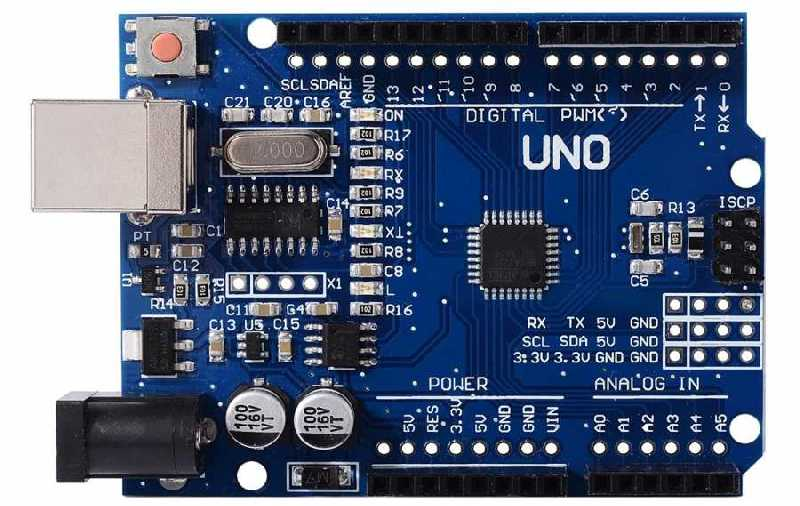
\includegraphics[width=.75\textwidth]{figures/arduino10.jpg}}
  \caption{Ini adalah Arduino}
  \label{fig:arduino}
  \end{figure}

 2. LED 5mm Bening pada gambar \ref{fig:led}
  \begin{figure}[ht]
  \centerline{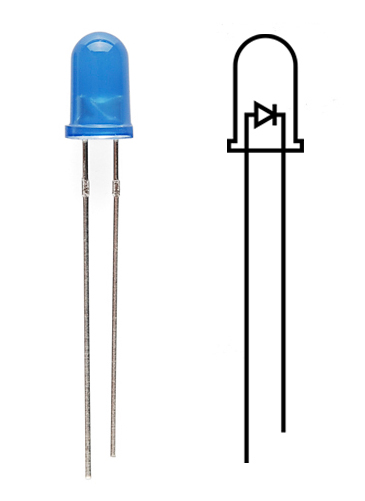
\includegraphics[width=.75\textwidth]{figures/led10.jpg}}
  \caption{Ini adalah Led}
  \label{fig:led}
  \end{figure}

 3. Bread Board
 \ref{fig:brb}
  \begin{figure}[ht]
  \centerline{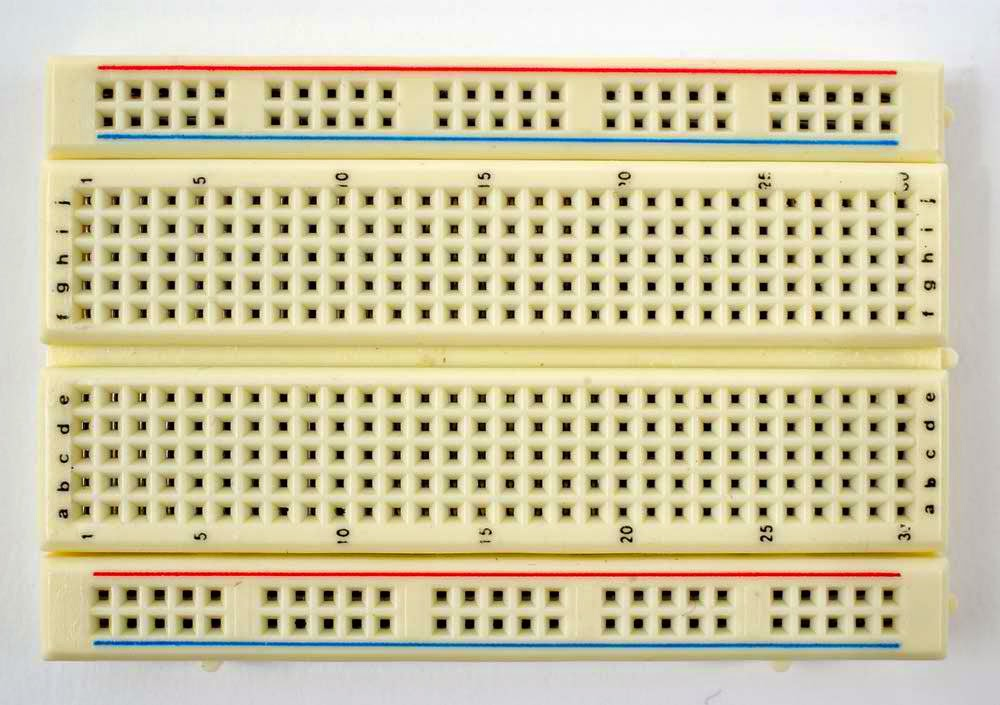
\includegraphics[width=.75\textwidth]{figures/brb.jpg}}
  \caption{Ini adalah BreadBoard}
  \label{fig:brb}
  \end{figure}

 4. Kabel Jumper pada gambar \ref{fig:jumper}.
  \begin{figure}[ht]
  \centerline{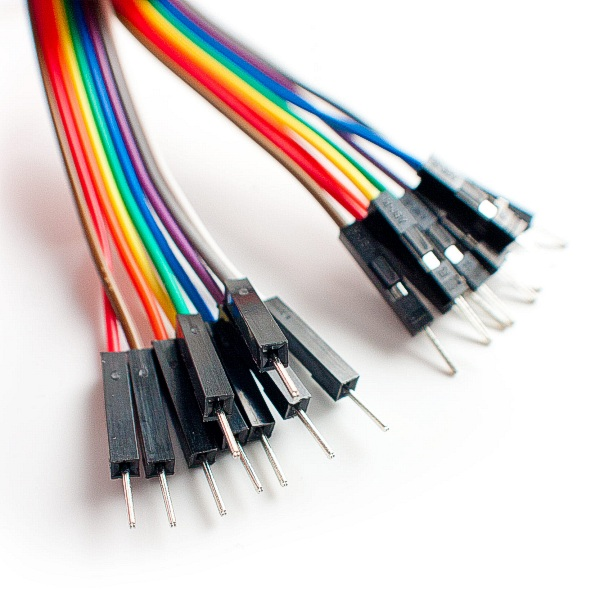
\includegraphics[width=.75\textwidth]{figures/jumper.jpg}}
  \caption{Ini adalah Kabel Jumper}
  \label{fig:jumper}
  \end{figure}

 5. Software IDE Arduino pada gambar \ref{fig:ide}
  \begin{figure}[ht]
  \centerline{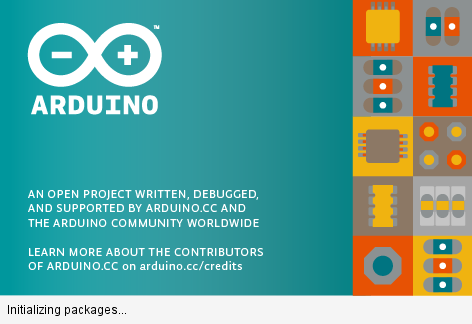
\includegraphics[width=.75\textwidth]{figures/ide.png}}
  \caption{Ini adalah Software IDE}
  \label{fig:ide}
  \end{figure}

\section{Membuat Perancangan}

Membuat perancangan dapat dilakukan dengan menggunakan bantuan arduino simulator misalnya VBB (Virtual Bread Board). Langkah installasinya yaitu;
1. Download aplikasi VBB,
2. Install,
    a. Double click installer VBB seperti pada gambar;
\begin{figure}[ht]
  \centerline{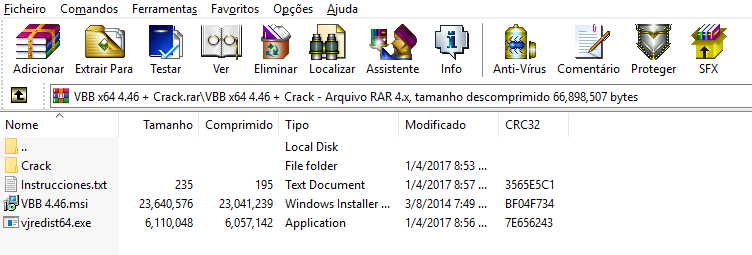
\includegraphics[width=.75\textwidth]{figures/installer.png}}
  \caption{Ini adalah installer vbb}
  \label{fig:installer}
  \end{figure}
    b. maka akan muncul seperti pada gambar;
\begin{figure}[ht]
  \centerline{\includegraphics[width=.75\textwidth]{figures/halawalinstall.png}}
  \caption{Ini adalah halaman awal penginstallan vbb}
  \label{fig:halawalinstall}
  \end{figure}
    c. lalu pilih next, seperti pada gambar;
\begin{figure}[ht]
  \centerline{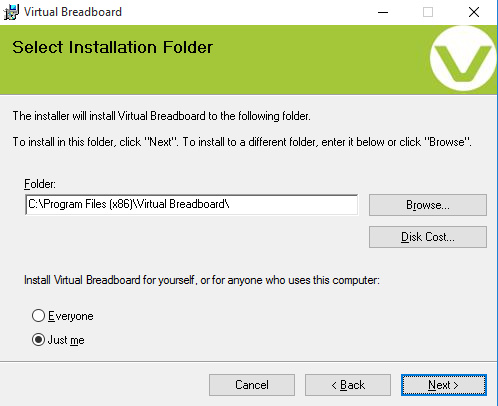
\includegraphics[width=.75\textwidth]{figures/memilihdirektori.png}}
  \caption{Ini adalah halaman untuk memilih direktori}
  \label{fig:memilihdirektori}
  \end{figure}
    d. lalu konfirmasi install dengan next, seperti pada gambar;
\begin{figure}[ht]
  \centerline{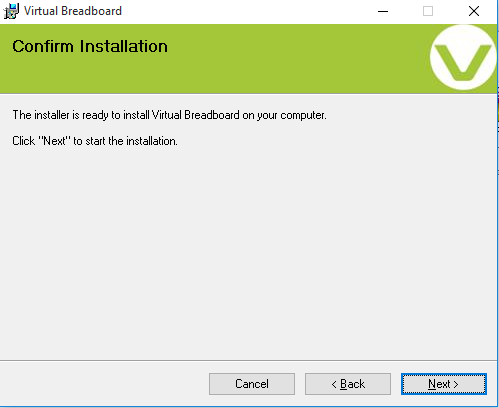
\includegraphics[width=.75\textwidth]{figures/konfirmasiinstall.png}}
  \caption{Ini adalah halaman konfirmasi installasi}
  \label{fig:konfirmasiinstall}
  \end{figure}
    e. proses installasi, seperti pada gambar;
\begin{figure}[ht]
  \centerline{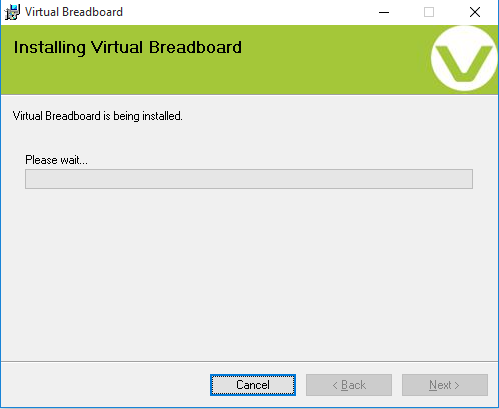
\includegraphics[width=.75\textwidth]{figures/prosesinstallasi.png}}
  \caption{Ini adalah halaman proses installasi}
  \label{fig:prosesinstallasi}
  \end{figure}
    f. installasi selesai, seperti pada gambar;
\begin{figure}[ht]
  \centerline{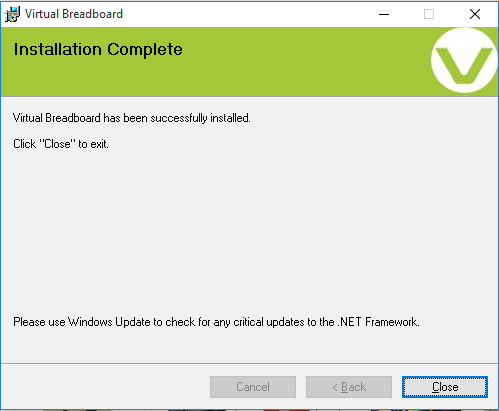
\includegraphics[width=.75\textwidth]{figures/installasiselesai.png}}
  \caption{Ini adalah proses installasi selesai}
  \label{fig:installasiselesai}
  \end{figure}
  
\section{Merancang Menggunakan VBB}
Langkah perancangannya adalah sebagai berikut;
1. Buka Aplikasi VBB (Virtual Bread Board), seperti pada gambar;
\begin{figure}[ht]
  \centerline{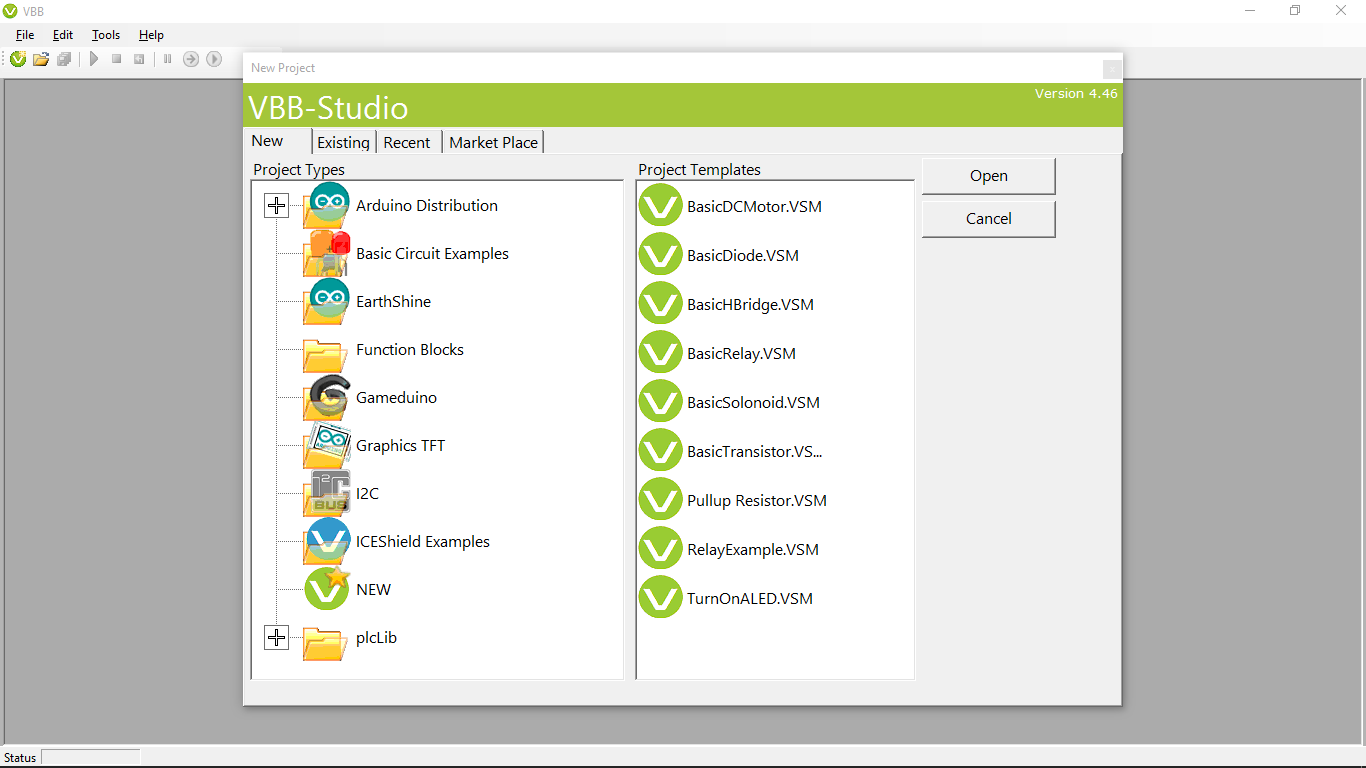
\includegraphics[width=.75\textwidth]{figures/bukaaplikasi.png}}
  \caption{Ini adalah aplikasi VBB}
  \label{fig:bukaaplikasi}
  \end{figure}
2. Pilih New Project,
\begin{figure}[ht]
  \centerline{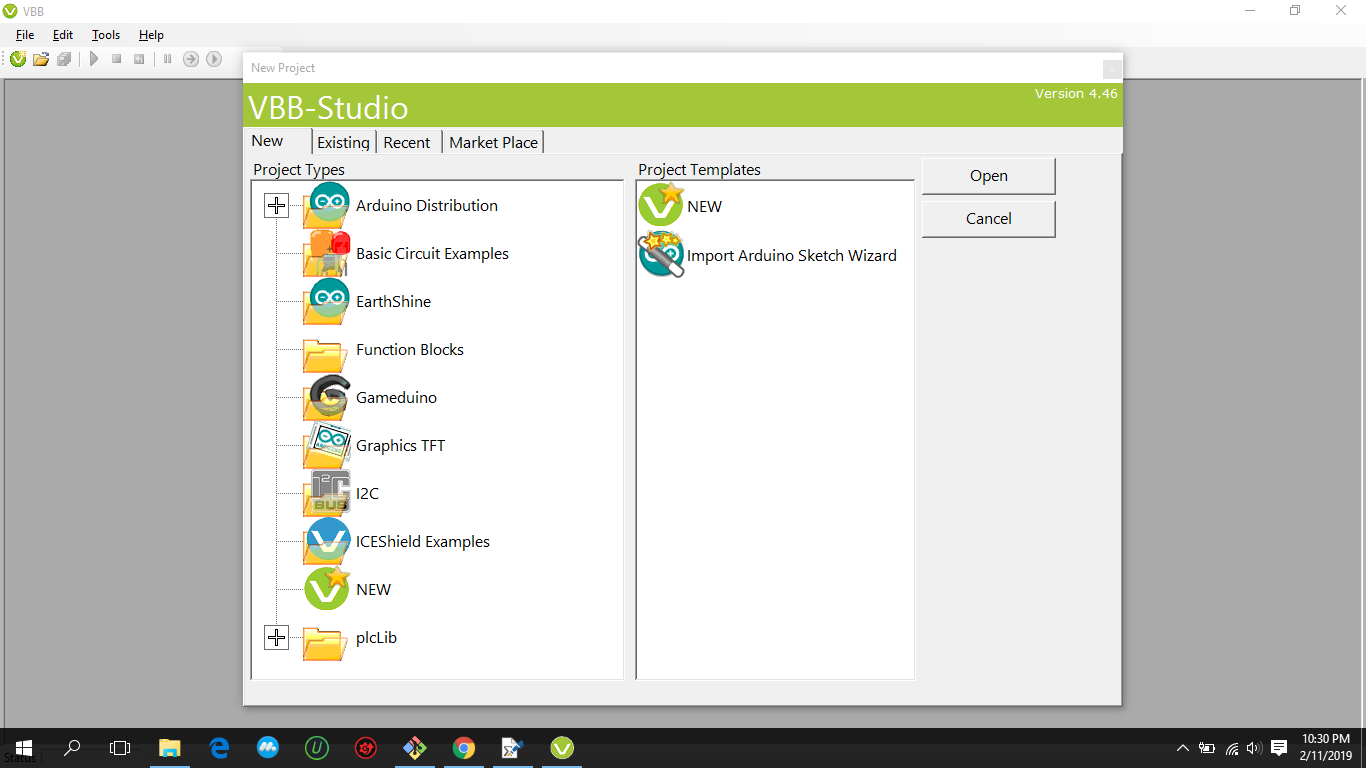
\includegraphics[width=.75\textwidth]{figures/newproject.png}}
  \caption{pilih new project}
  \label{fig:newproject}
  \end{figure}
3. Lalu pilih perangkat apa saja yang dibutuhkan, seperti pada gambar;
\begin{figure}[ht]
  \centerline{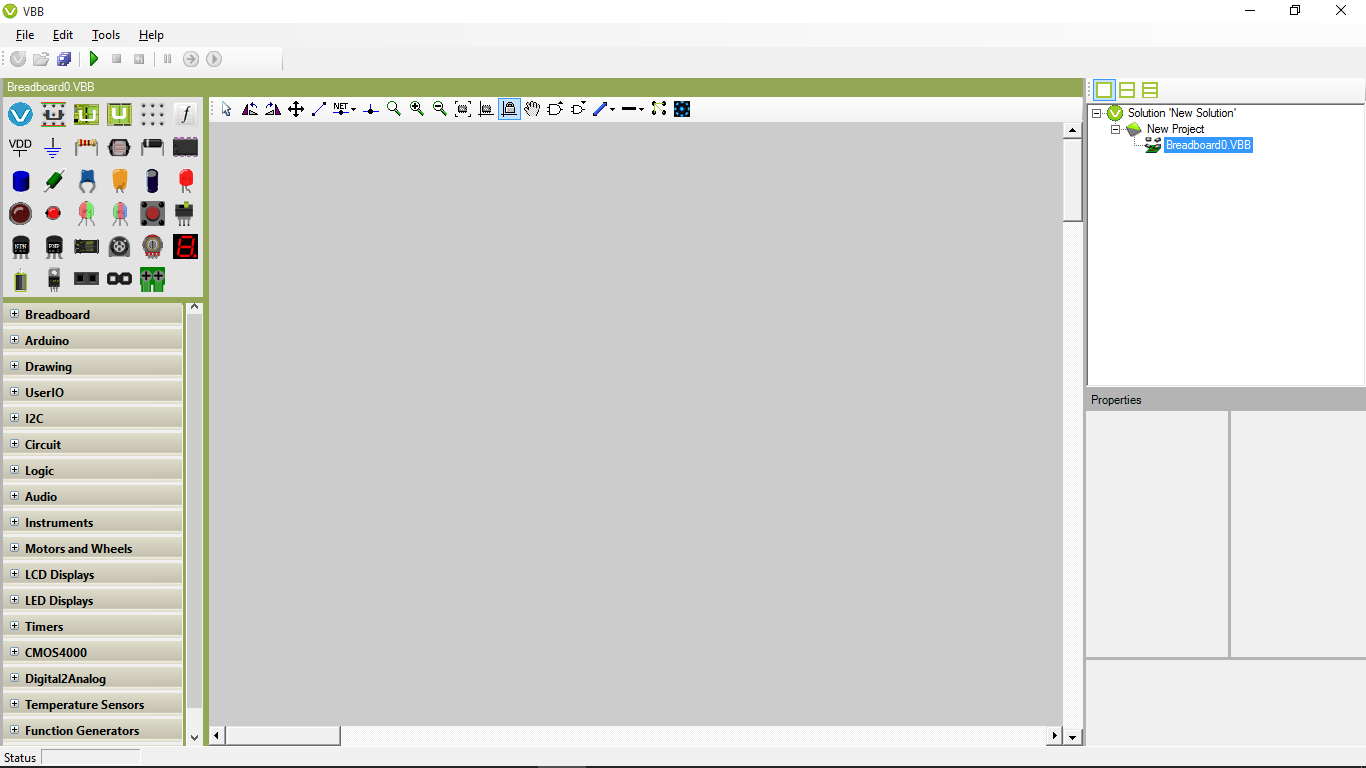
\includegraphics[width=.75\textwidth]{figures/halvbb.png}}
  \caption{Ini adalah Halaman project baru VBB}
  \label{fig:halvbb}
  \end{figure}
\section{Proses Pembuatan}

1. Download dan Instal aplikasi IDE

2.Rakit semua alat menjadi satu kesatuan

  gambar \ref{ar2} adalah....
  \begin{figure}[ht]
  \centerline{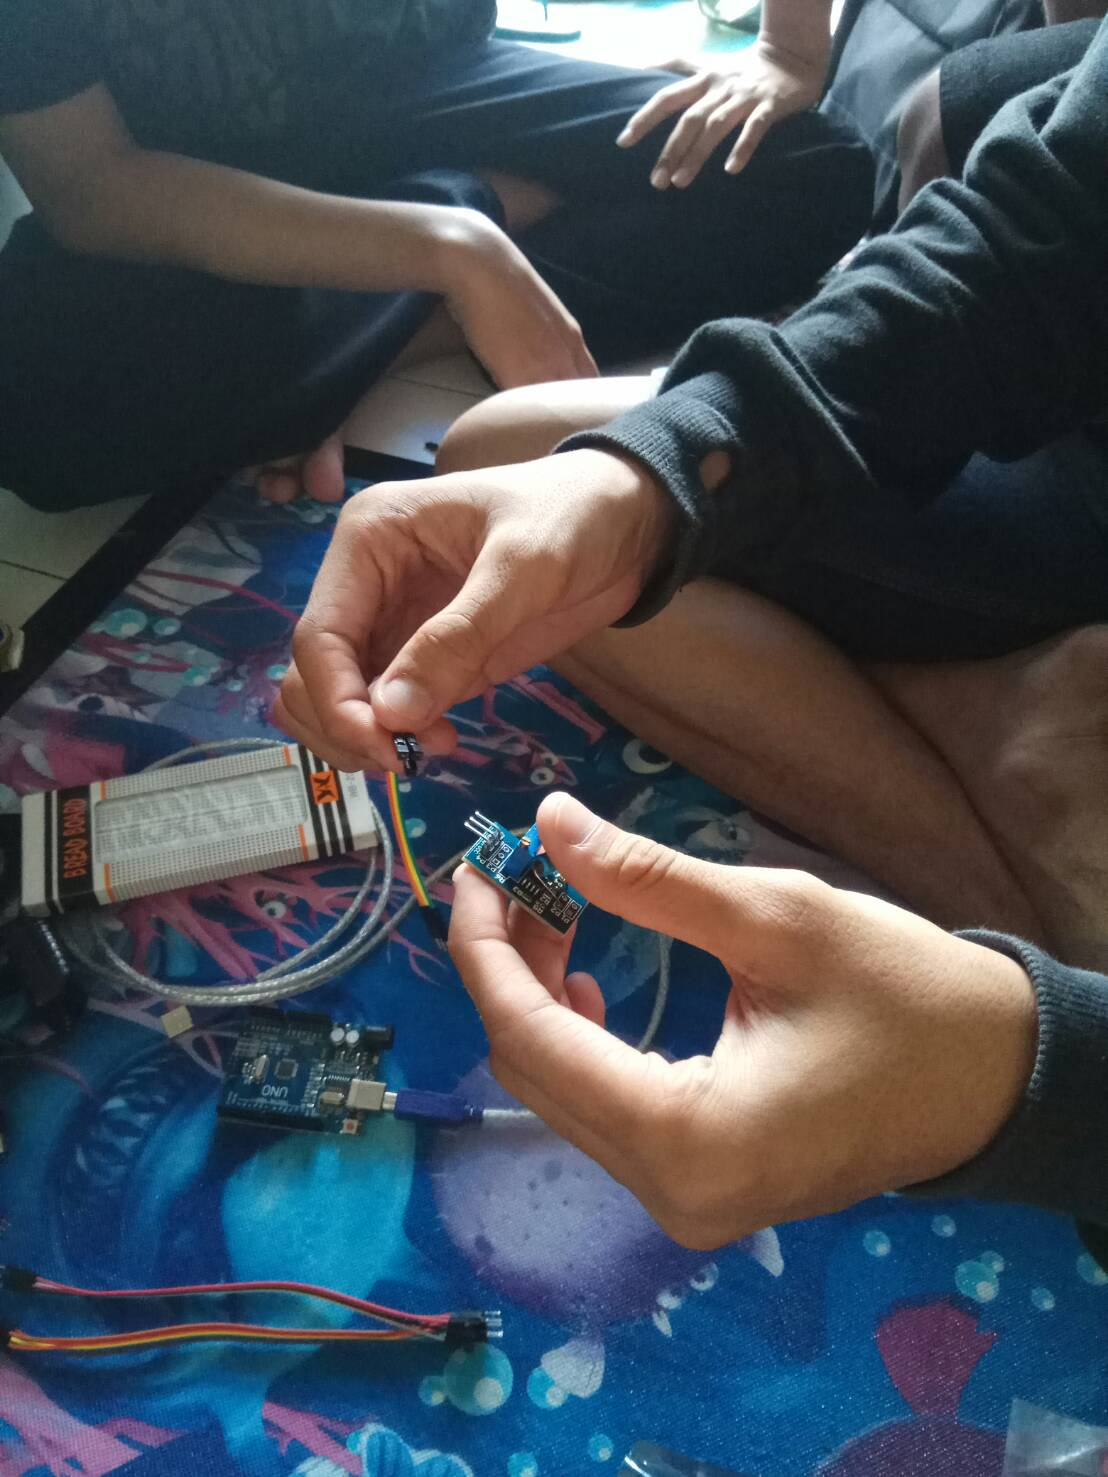
\includegraphics[width=.75\textwidth]{figures/ar2.jpg}}
  \caption{Ini adalah Proses Perakitan}
  \label{ar2}
  \end{figure}

  gambar \ref{ar3}adalah....
  \begin{figure}[ht]
  \centerline{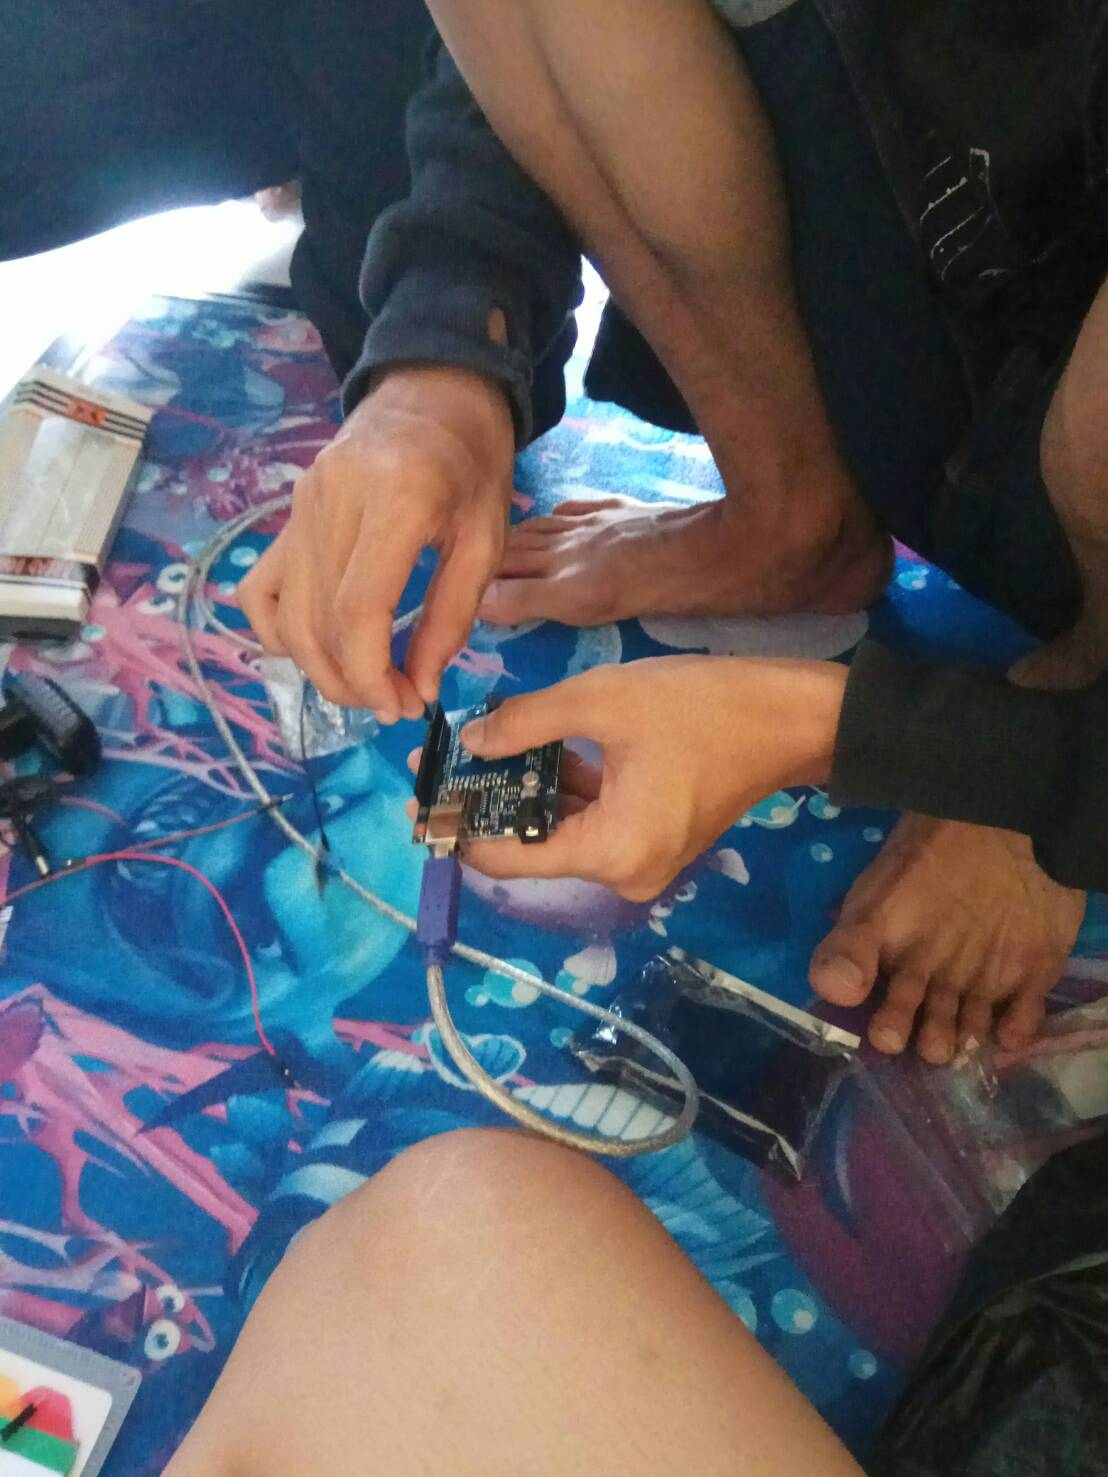
\includegraphics[width=.75\textwidth]{figures/ar3.jpg}}
  \caption{Ini adalah Proses Perakitan}
  \label{ar3}
  \end{figure}

  gambar \ref{ar4}adalah....
  \begin{figure}[ht]
  \centerline{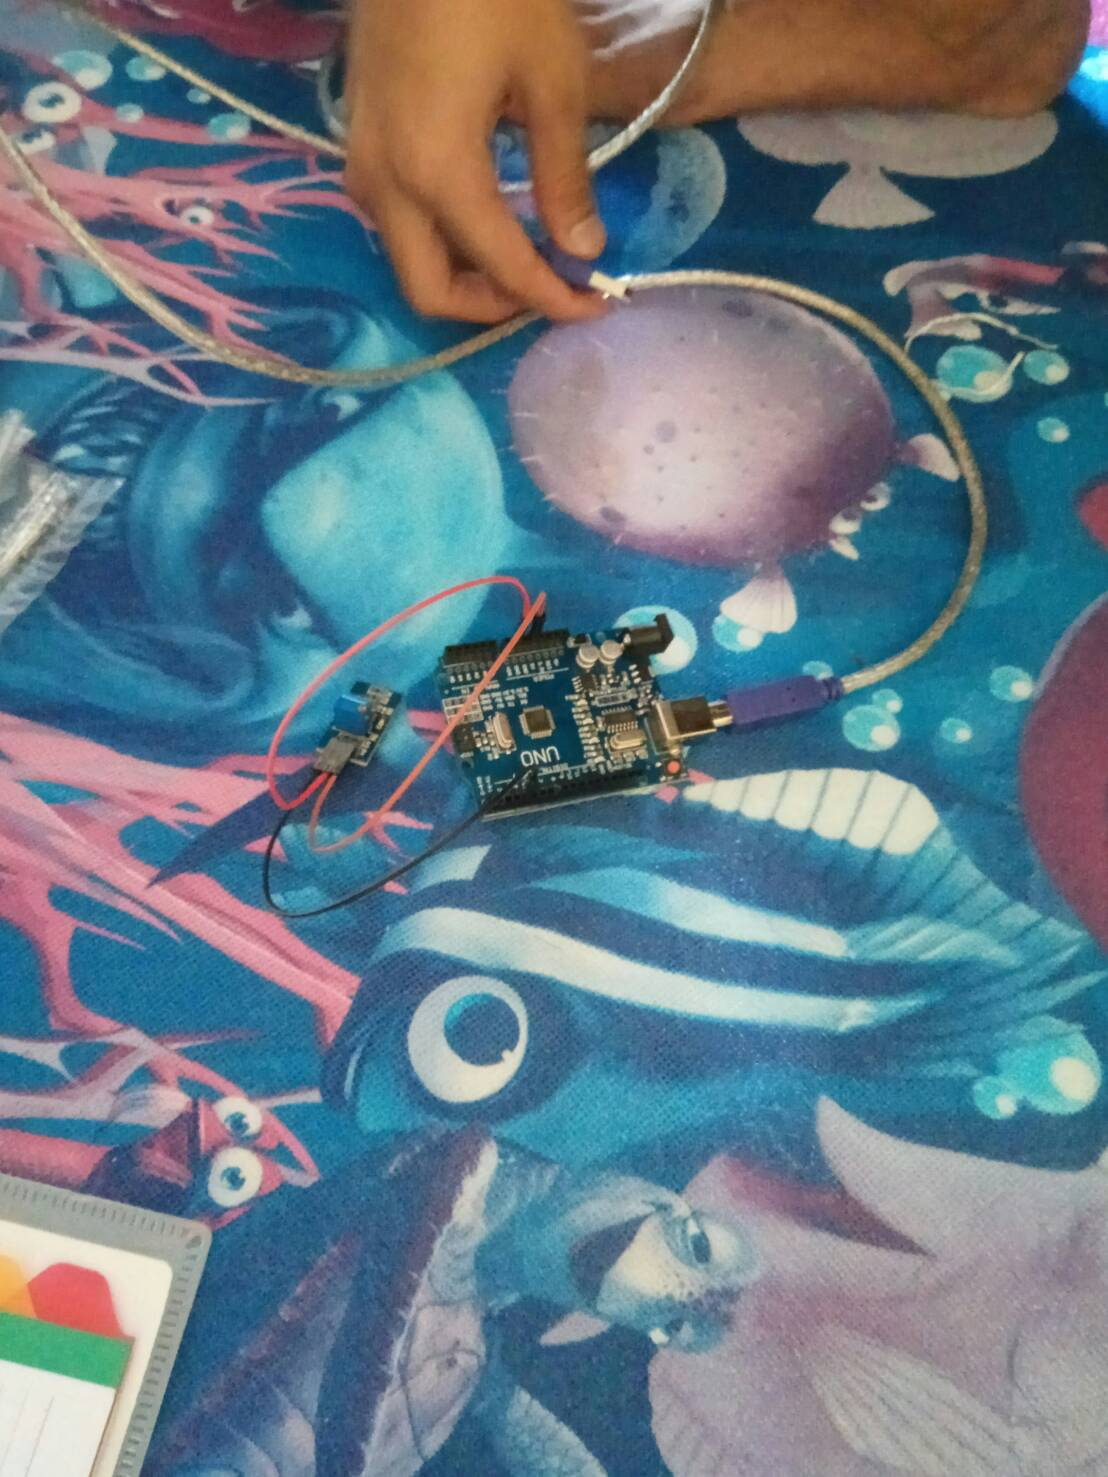
\includegraphics[width=.75\textwidth]{figures/ar4.jpg}}
  \caption{Ini adalah Proses Perakitan}
  \label{ar4}
  \end{figure}

  gambar \ref{ar5}adalah....
  \begin{figure}[ht]
  \centerline{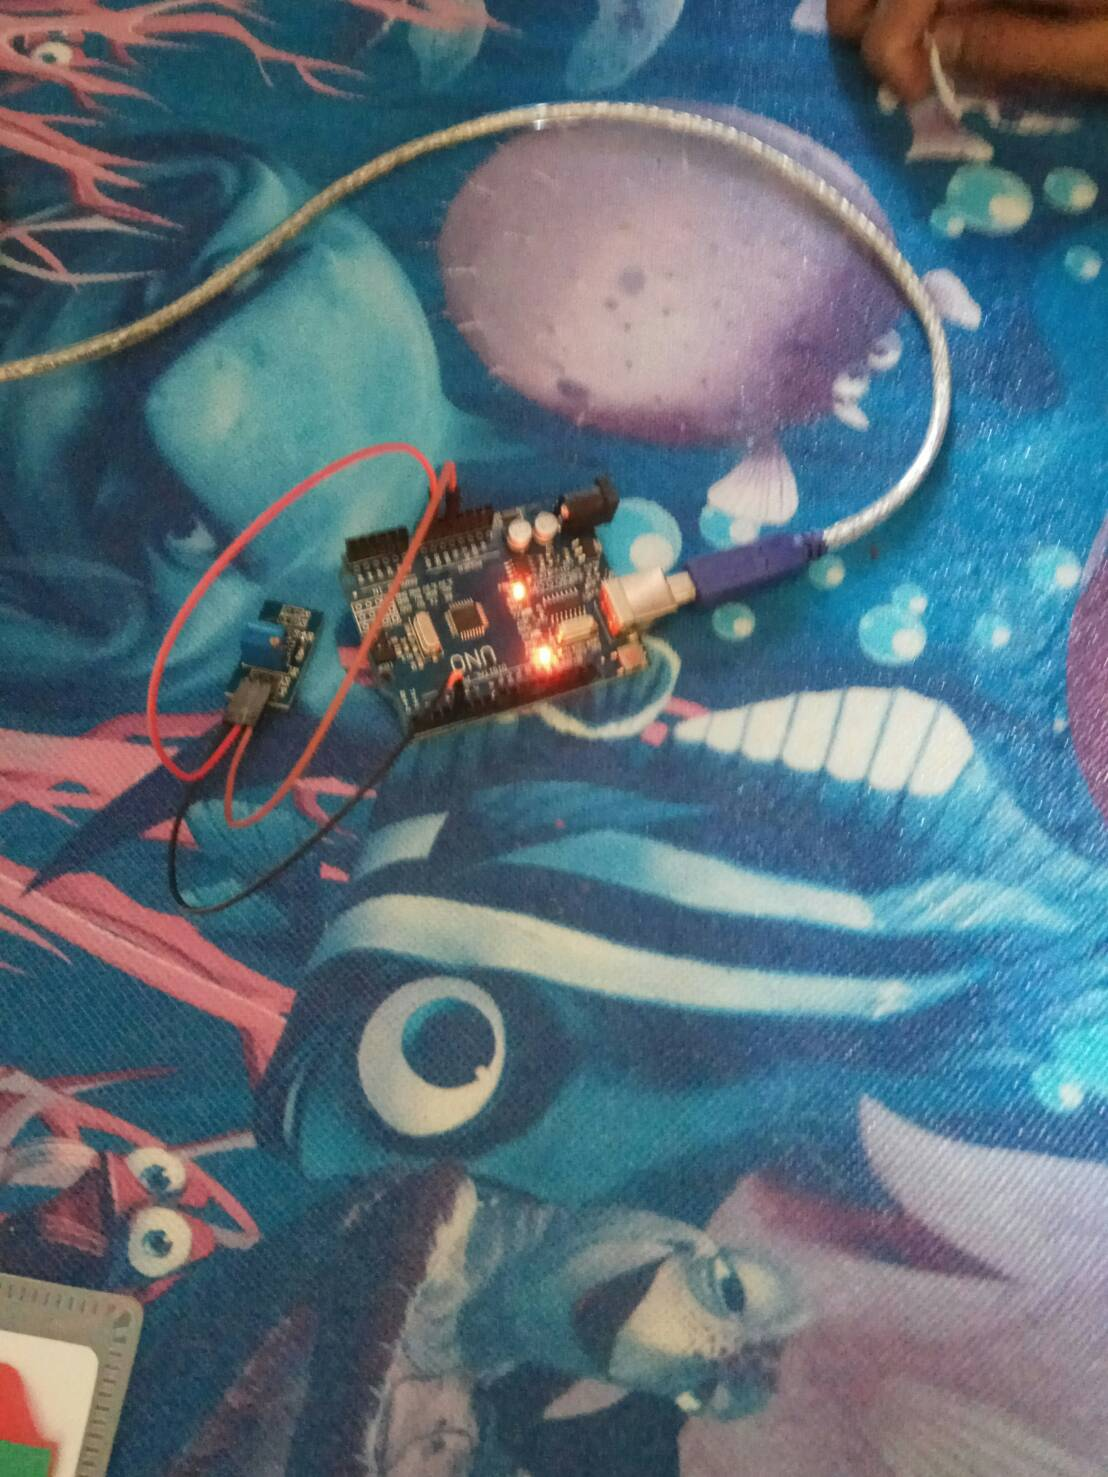
\includegraphics[width=.75\textwidth]{figures/ar5.jpg}}
  \caption{Ini adalah Proses Perakitan}
  \label{ar5}
  \end{figure}

 gambar \ref{ar6}adalah....
  \begin{figure}[ht]
  \centerline{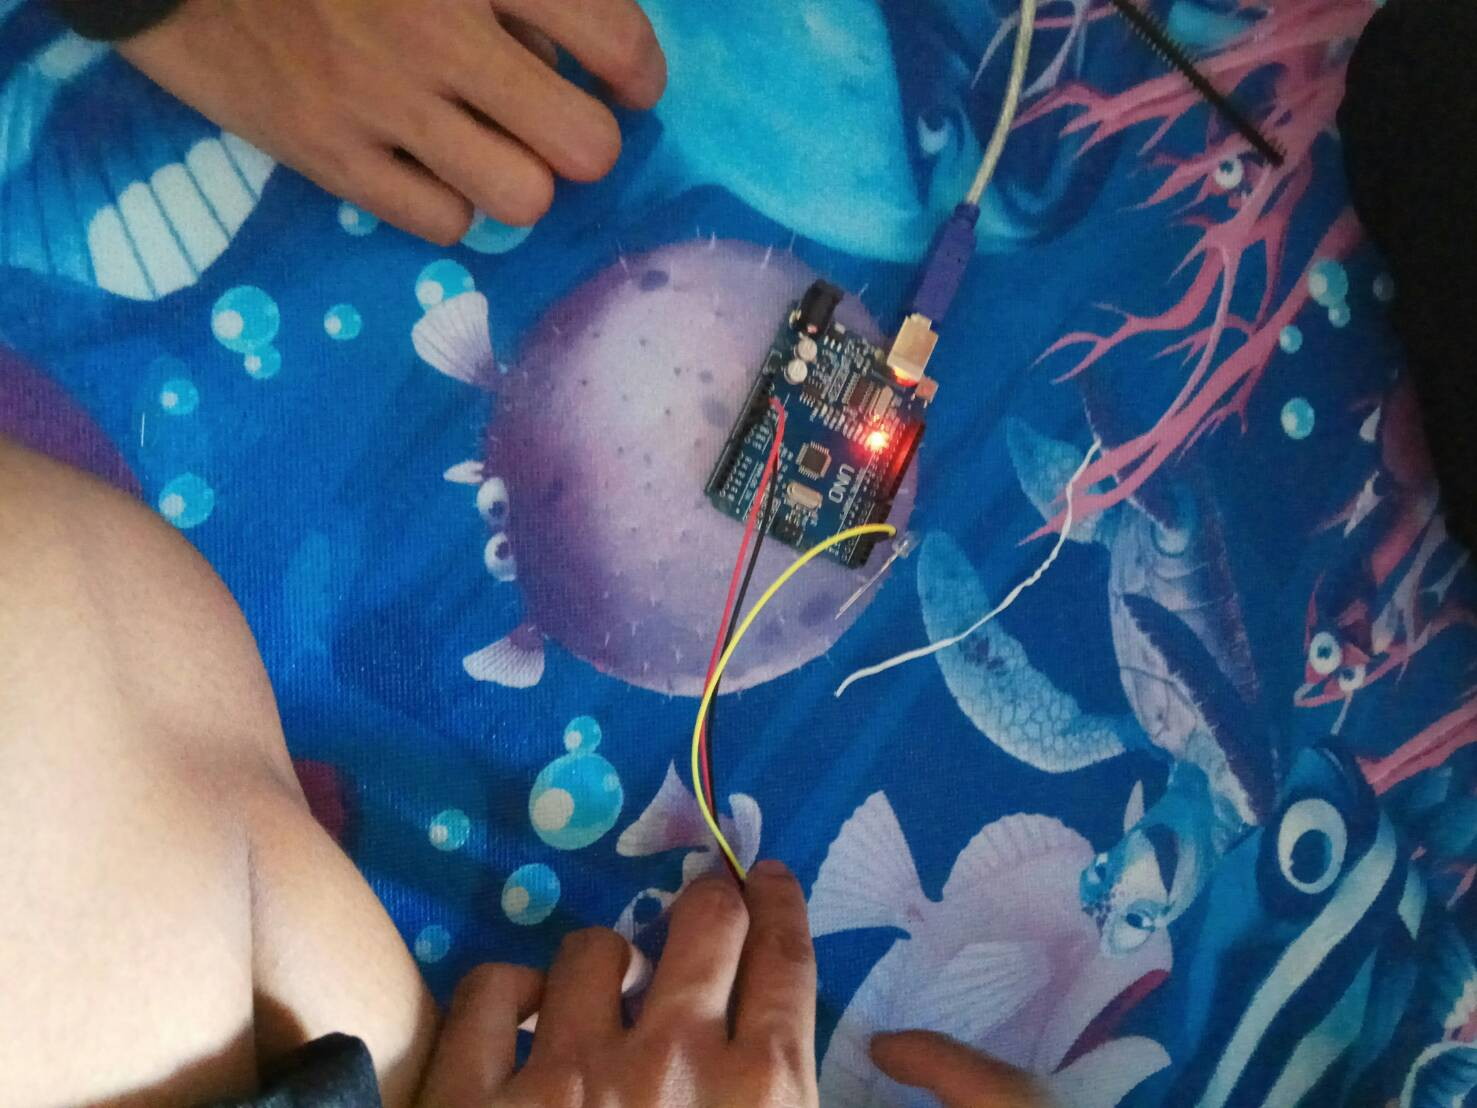
\includegraphics[width=.75\textwidth]{figures/ar6.jpg}}
  \caption{Ini adalah Proses Perakitan}
  \label{ar6}
  \end{figure}

 3. Sambungkan Kabel Printer dengan Laptop seperti gambar \ref{ar7}.
  \begin{figure}[ht]
  \centerline{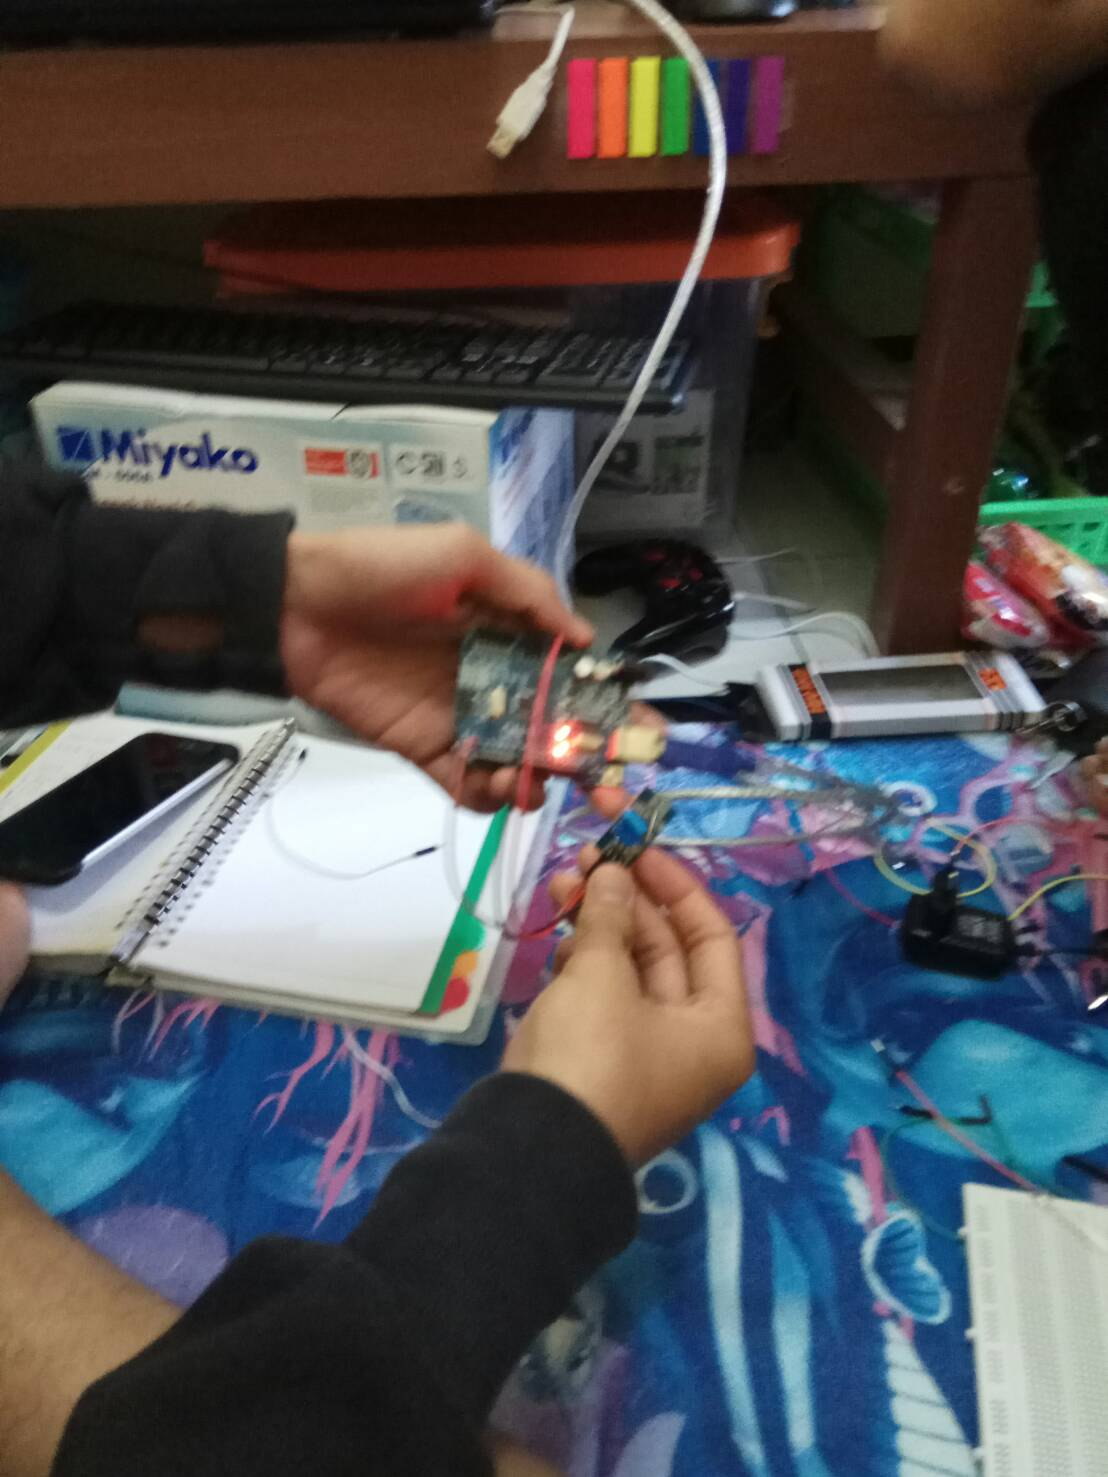
\includegraphics[width=.75\textwidth]{figures/ar7.jpg}}
  \caption{Ini adalah Proses Penyambungan}
  \label{ar7}
  \end{figure}

 4. Lakukan Pengodingan di IDE seperti pada gambar \ref{ar8}
  \begin{figure}[ht]
  \centerline{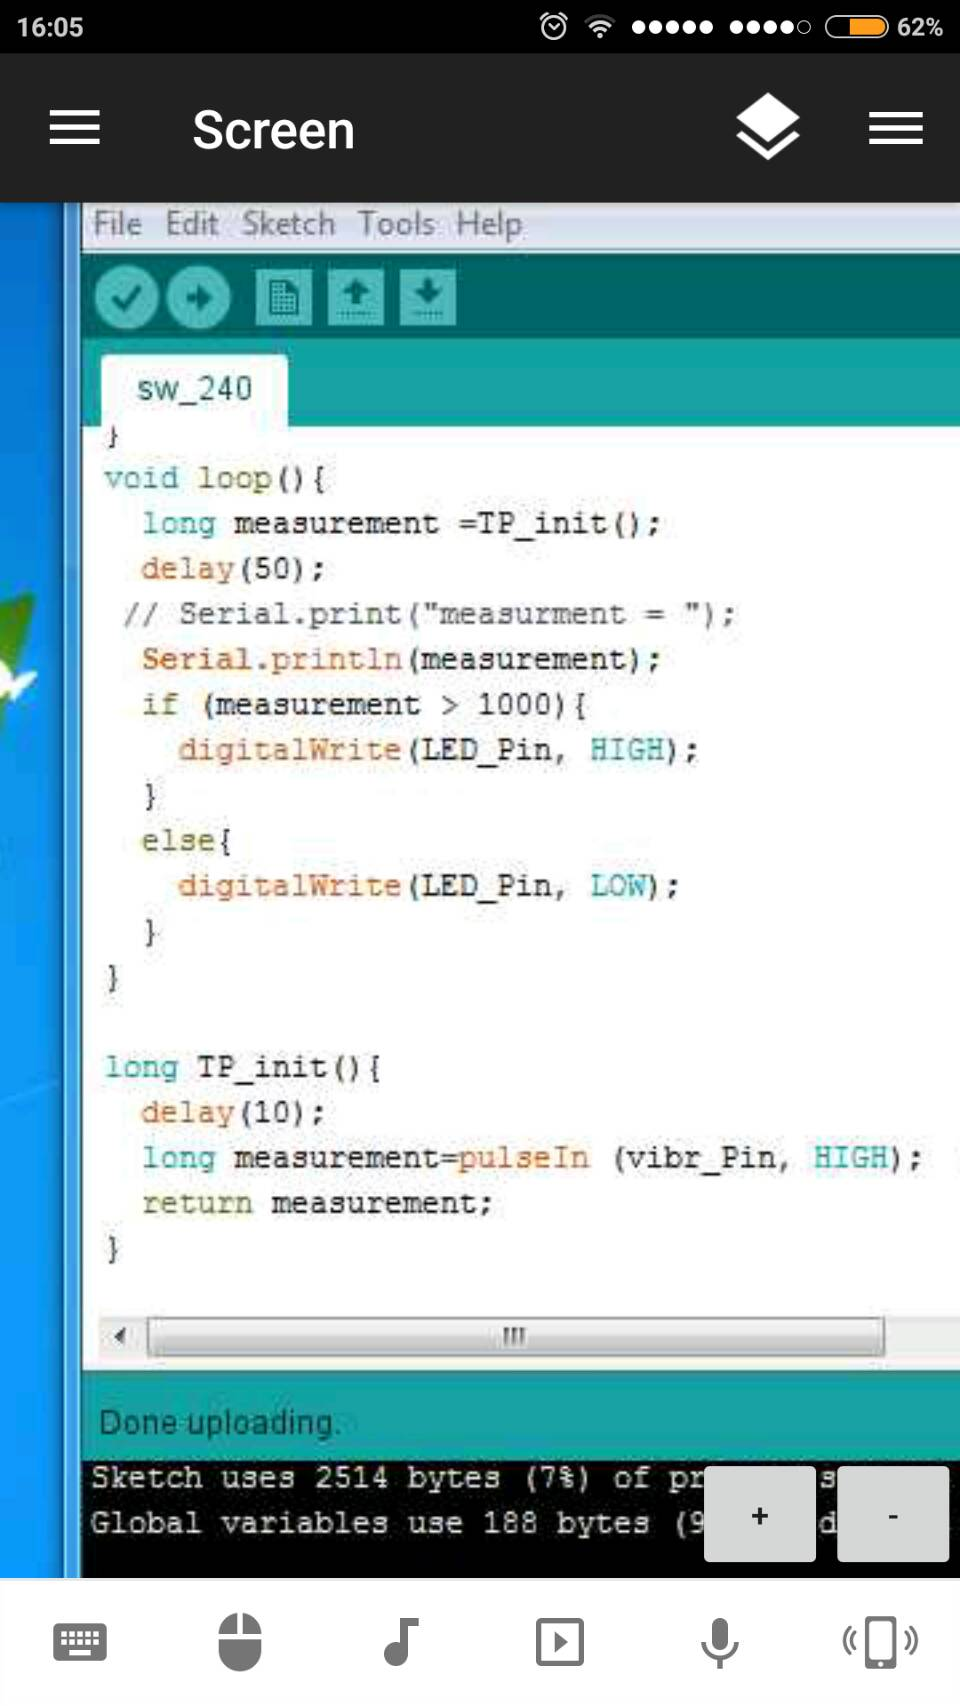
\includegraphics[width=.75\textwidth]{figures/ar8.jpg}}
  \caption{Ini adalah Proses Pengodingan}
  \label{ar8}
  \end{figure}

																											